\uuid{wKNW}
\exo7id{5473}
\titre{exo7 5473}
\auteur{rouget}
\organisation{exo7}
\datecreate{2010-07-10}
\isIndication{false}
\isCorrection{true}
\chapitre{Intégration}
\sousChapitre{Intégrale de Riemann dépendant d'un paramètre}
\module{Analyse}
\niveau{L2}
\difficulte{}

\contenu{
\texte{
Etude de $f(x)=\int_{0}^{1}\mbox{Max}(x,t)\;dt$.
}
\reponse{
Soit $x\in\Rr$. La fonction $t\mapsto\mbox{Max}(x,t)=\frac{1}{2}(x+t+|x-t|)$ est continue sur $[0,1]$ en vertu de théorèmes généraux. Par suite, $\int_{0}^{1}\mbox{Max}(x,t)\;dt$ existe. 

Si $x\leq0$, alors $\forall t\in[0,1]$, $x\leq t$ et donc $\mbox{Max}(x,t)=t$. Par suite, $f(x)=\int_{0}^{1}t\;dt=\frac{1}{2}$.

Si $x\geq1$, alors $\forall t\in[0,1]$, $t\leq x$ et donc $\mbox{Max}(x,t)=x$. Par suite, $f(x)=\int_{0}^{1}x\;dt=x$.

Si $0<x<1$,

$$f(x)=\int_{0}^{x}x\;dt+\int_{x}^{1}t\;dt=x^2+\frac{1}{2}(1-x^2)=\frac{1}{2}(1+x^2).$$

En résumé, $\forall x\in\Rr,\;f(x)=\left\{
\begin{array}{l}
\frac{1}{2}\;\mbox{si}\;x\leq0\\
\frac{1}{2}(1+x^2)\;\mbox{si}\;0<x<1\\
x\;\mbox{si}\;x\geq1
\end{array}
\right.$.

$f$ est déjà continue sur $]-\infty,0]$, $[1,+\infty[$ et $]0,1[$. De plus, $f(0^+)=\frac{1}{2}=f(0)$ et $f(1^-)=1=f(1)$. $f$ est ainsi continue à droite en $0$ et continue à gauche en $1$ et donc sur $\Rr$.

$f$ est de classe $C^1$ sur $]-\infty,0]$, $[1,+\infty[$ et $]0,1[$. De plus, $\lim_{x\rightarrow 0,\;x>0}f'(x)=\lim_{x\rightarrow 0,\;x>0}x=0$. $f$ est donc continue sur $[0,1[$ de classe $C^1$ sur $]0,1[$ et $f'$ a une limite réelle quand $x$ tend vers $0$. D'après un théorème classique d'analyse, $f$ est de classe $C^1$ sur $[0,1[$ et en particulier, $f$ est dérivable à droite en $0$ et ${f'}_{d}(0)=0$. Comme d'autre part, $f$ est dérivable à gauche en $0$ et que ${f'}_{g}(0)=0={f'}_{d}(0)$, $f$ est dérivable en $0$ et $f'(0)=0$.

L'étude en $1$ montre que $f$ est dérivable en $1$ et que $f'(1)=1$. Le graphe de $f$ est le suivant~:

$$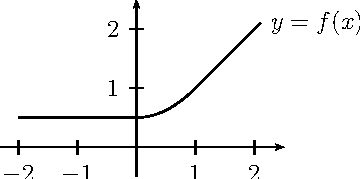
\includegraphics{../images/pdf/wKNW-1.pdf}$$
}
}
